\documentclass{article}
\usepackage{amsmath}
\usepackage{amssymb}
\usepackage{graphicx}
\usepackage{geometry}
\geometry{a4paper, margin=1in}

\title{Documentation: Simulation of Observable Effects of Cluster Member Speed Increase}
\author{Mohammadali Taefi}
\date{\today}

\begin{document}
	
	\maketitle
	
	\section{Introduction}
	
	\subsection{Purpose}
	
	This code simulates an open star cluster and surrounding field stars to model and visualize the observable effects (from Earth) of reducing the speed of cluster member stars. 
	
	\subsection{Relevance}
	
	Understanding the dynamics of star clusters and how internal velocity changes manifest in observable parameters (like proper motion, radial velocity) is crucial in astrophysics. Gaia observations provide precise astrometric and kinematic data, making such simulations essential for interpreting real-world observations.
	
	\subsection{Presumptions}
	
	\begin{itemize}
		\item The simulation simplifies the complex gravitational interactions within a star cluster.
		\item Initial conditions (spatial and velocity distributions) significantly influence the outcome.
		\item The observer (Earth) is far enough from the cluster to apply certain geometric approximations.
	\end{itemize}
	
	\section{Code Description}
	
	\subsection{Star Generation}
	
	\subsubsection{Cluster Stars}
	
	\paragraph{Spatial Distribution}
	
	The code uses a Plummer model to generate the initial spatial distribution of cluster stars. This model is chosen to represent a typical density profile of star clusters, with a higher density of stars towards the center.
	
	\paragraph{Velocity Distribution}
	
	Cluster stars are assigned velocities drawn from a Gaussian distribution. The mean and dispersion of this distribution are parameters that can be adjusted. 
	
	\paragraph{Justification}
	
	The Plummer model provides a reasonable approximation of the spatial structure of many observed open clusters. The Gaussian velocity distribution is a common assumption in the absence of more specific knowledge about the cluster's dynamical history.
	
	\subsubsection{Field Stars}
	
	\paragraph{Spatial Distribution}
	
	Field stars are generated randomly within a defined cubic volume. This represents the general background population of stars in the galaxy.
	
	
	
	\paragraph{Justification}
	
	Random spatial distribution is a simplified representation of the field star distribution. 
	
	\subsection{Speed Modification}
	
	The code includes functionality to modify the velocities of cluster members. 
	
	\subsubsection{Constant Speed Addition}
	
	Adds a constant velocity vector pointing radially outwards from the cluster center to each cluster member. 
	
	\subsubsection{Gaussian Speed Addition}
	
	Adds a velocity component whose magnitude follows a Gaussian distribution with respect to the distance from the cluster center (stars closer to the center have a larger additional speed).
	
	\subsubsection{Justification}
	
	These modifications allow for exploration of how different velocity profiles within a cluster affect its observed properties. For example, the Gaussian speed addition could mimic the effect of dynamical processes that preferentially accelerate stars near the cluster's core.
	
	\subsection{Coordinate Transformation}
	
	The code transforms the simulated spatial and velocity data into observable coordinates (Right Ascension, Declination, parallax, proper motion, radial velocity) as seen from Earth. 
	
	This transformation takes into account:
	
	\begin{itemize}
		\item The distance and location of the cluster center relative to Earth. 
		\item The motion of the cluster center relative to Earth. 
	\end{itemize}
	
	\paragraph{Justification}
	
	This is essential to connect the simulated intrinsic properties of the cluster to what astronomers actually measure.
	
	\subsection{Observable Calculations}
	
	\begin{itemize}
		\item Parallax: Calculated from the distance of each star. 
		\item Proper Motion: Calculated from the transverse velocities of the stars. 
		\item Radial Velocity: Calculated from the component of the star's velocity along the line of sight. 
	\end{itemize}
	
	\paragraph{Justification}
	
	These are the fundamental observables used to study the kinematics of star clusters.
	
	\subsection{Visualization}
	
	The code generates plots to visualize: 
	
	\begin{itemize}
		\item Spatial distribution of stars. 
		\item Velocity distribution. 
		\item Proper motion vectors. 
		\item Distribution of stars in observable coordinates (RA, Dec, parallax, radial velocity). 
	\end{itemize}
	
	\paragraph{Justification}
	
	Visualization is crucial for understanding the complex 3D data and for identifying patterns in the simulated observables.
	
	\section{Presumptions and Limitations}
	
	\begin{itemize}
		\item \textbf{Simplified Dynamics:} The simulation does \textit{not} include the gravitational interactions between stars. Stars are generated with initial positions and velocities, and their subsequent motion is not calculated. This is a major simplification, as gravity is the dominant force in star clusters.
		\item \textbf{Initial Conditions:} The results of the simulation are highly dependent on the initial spatial and velocity distributions. Different choices for the Plummer radius, velocity dispersion, etc., will lead to different observable properties. 
		\item \textbf{Observer Distance:} The code assumes that the observer (Earth) is located at a large distance from the cluster. This allows for the use of certain approximations in the coordinate transformations. 
		\item  \textbf{Coordinate System Alignment:} The simulation assumes a direct alignment between the simulation's Cartesian coordinates and the observer's coordinate system. In reality, a rotation would be needed.
		\item \textbf{Constant Velocity Modification:} The constant and Gaussian speed additions are artificial manipulations. They are not intended to represent realistic physical processes but rather to explore the \textit{sensitivity} of observable parameters to velocity changes.
	\end{itemize}
	
	\section{Procedure to Run the Code}
	
	\begin{itemize}
		\item The code is written in Python and requires libraries like NumPy, Pandas, and Matplotlib. 
		\item The user can modify various parameters, such as:
		\begin{itemize}
			\item Number of cluster and field stars. 
			\item Cluster size and density profile. 
			\item Cluster and field star velocity distributions. 
			\item Cluster distance and motion. 
			\item Parameters for the speed modification functions. 
		\end{itemize}
		\item The code outputs:
		\begin{itemize}
			\item A Pandas DataFrame containing the simulated stars and their properties (both in simulation coordinates and observable coordinates). 
			\item Various plots visualizing the spatial and velocity distributions of the stars. 
		\end{itemize}
	\end{itemize}
	
	\section{Expected Results and Interpretation}
	
	By comparing the observable properties of the simulated cluster \textit{with} and \textit{without} the speed modifications, the user can investigate:
	
	\begin{itemize}
		\item How changes in the internal velocities of cluster members affect the cluster's appearance on the sky (RA, Dec distribution). 
		\item How velocity changes influence the proper motion of cluster members. 
		\item Whether velocity changes have a significant impact on the parallax and radial velocity distributions. 
	\end{itemize}
	
	The plots of proper motion vectors are particularly important, as they can reveal the overall motion of the cluster and any internal kinematic structure. 
	
	The simulation can help to understand the challenges in interpreting real observational data and the importance of considering various factors that can affect the observed properties of star clusters.\\
	
	
The figures below illustrate three different states of a synthetic cluster, each with distinct speed conditions:
\begin{itemize}
	\item Default speed, as shown in Figure~\ref{fig:default}.
	\item A constant speed added to every member, depicted in Figure~\ref{fig:constant}.
	\item Speed added based on the position relative to the cluster center, presented in Figure~\ref{fig:Gaussian}.
\end{itemize}
	\begin{figure}[h] % 'h' places the figure approximately "here"
		\centering
		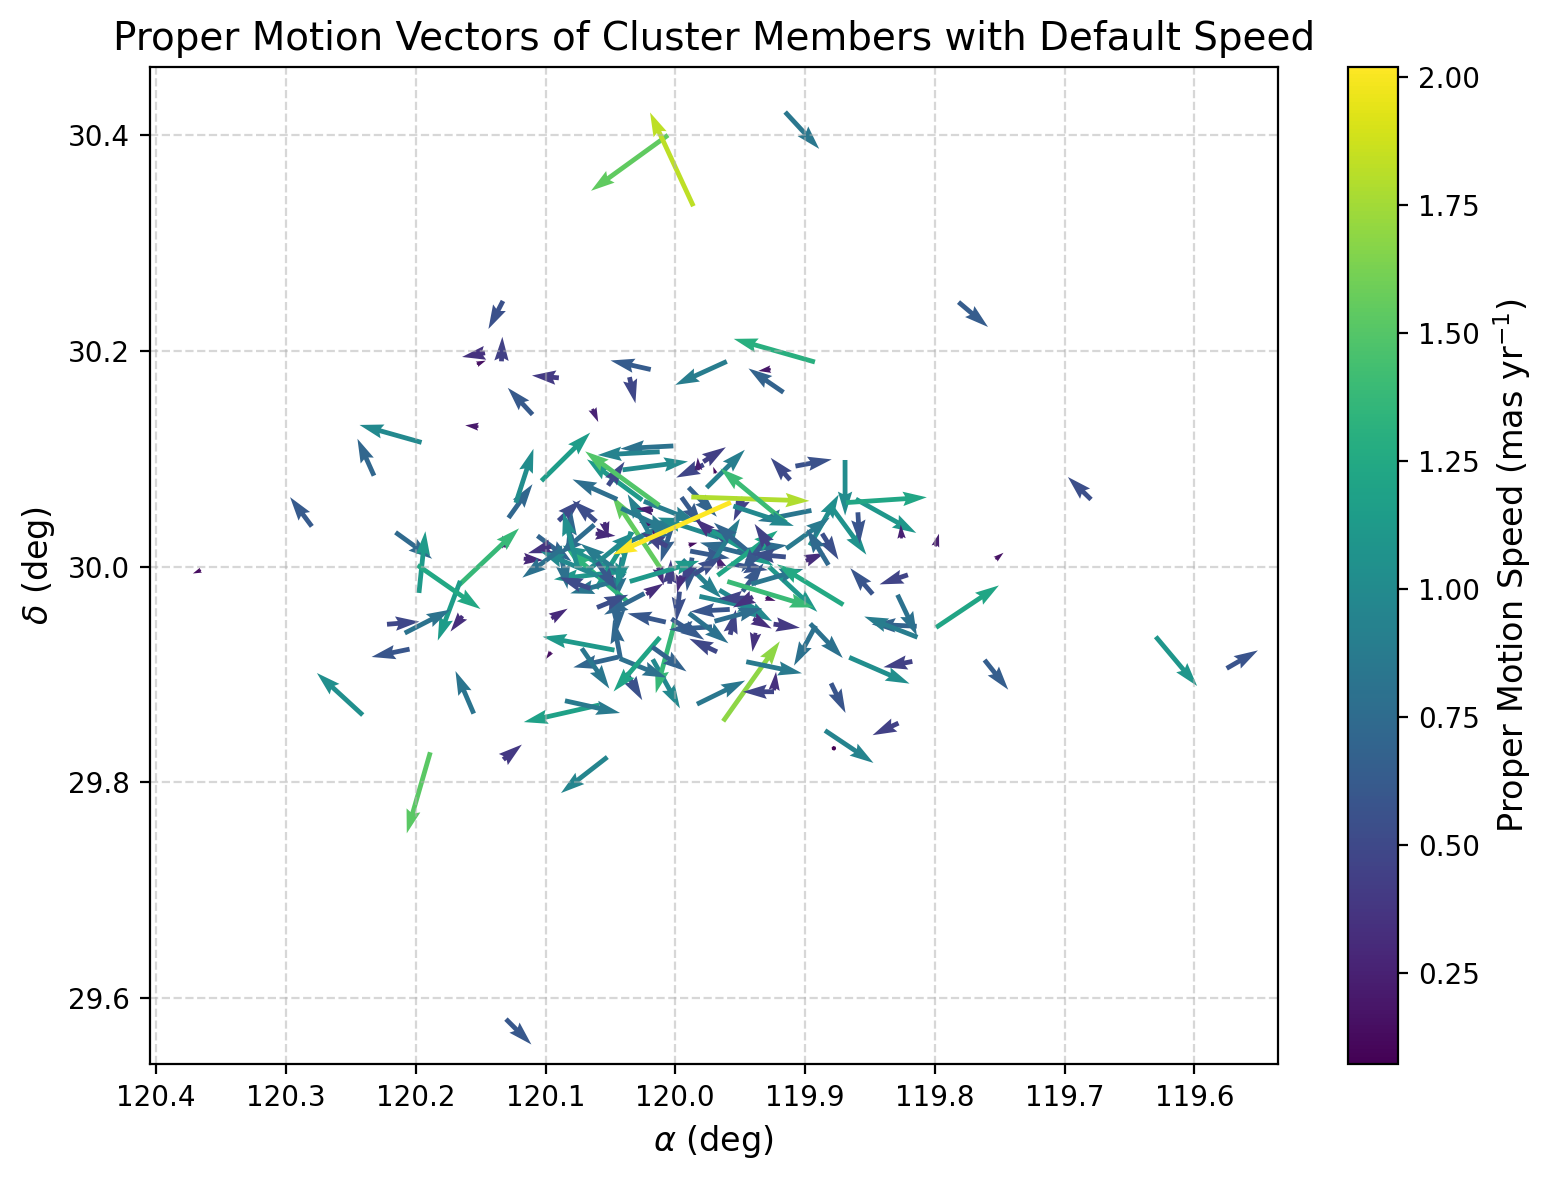
\includegraphics[width=0.5\textwidth]{default-speed.png} % Replace 'example-image' with your image file name
		\caption{} % Add your caption text here
		\label{fig:default} % Label for referencing the figure
	\end{figure}
	\begin{figure}[h] % 'h' places the figure approximately "here"
		\centering
		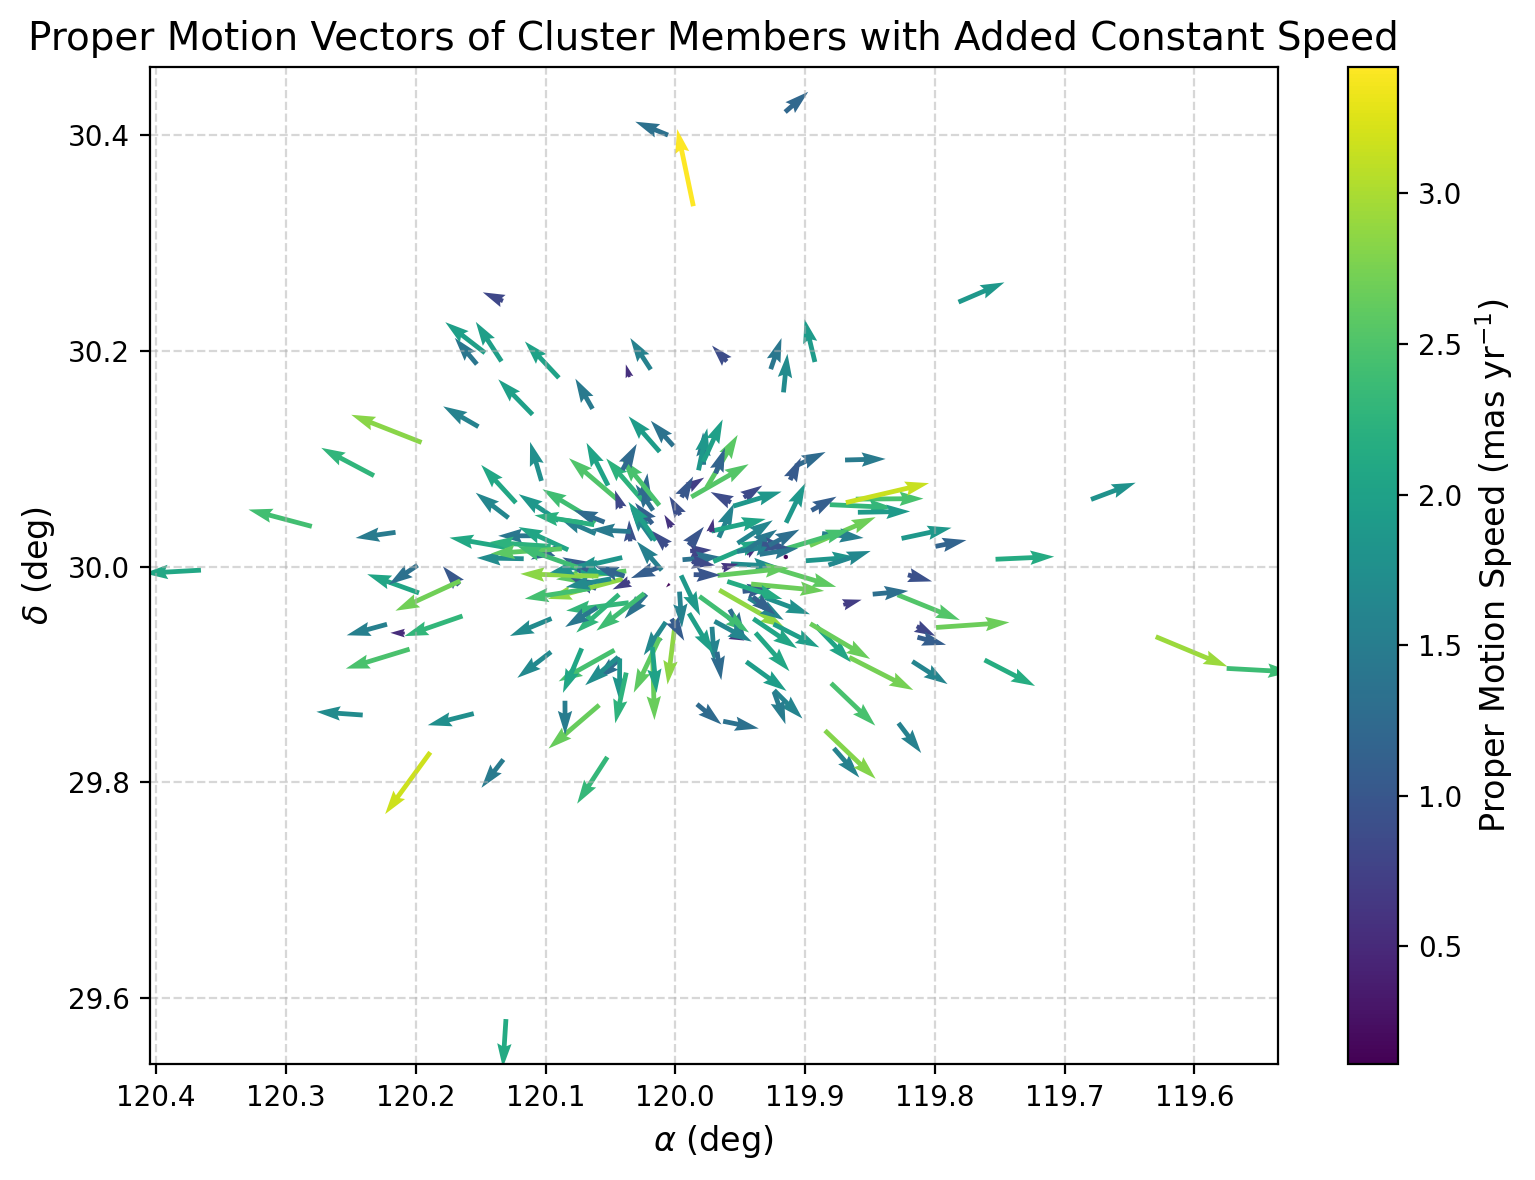
\includegraphics[width=0.5\textwidth]{constant-speed.png} % Replace 'example-image' with your image file name
		\caption{} % Add your caption text here
		\label{fig:constant} % Label for referencing the figure
	\end{figure}
	\begin{figure}[h] % 'h' places the figure approximately "here"
		\centering
		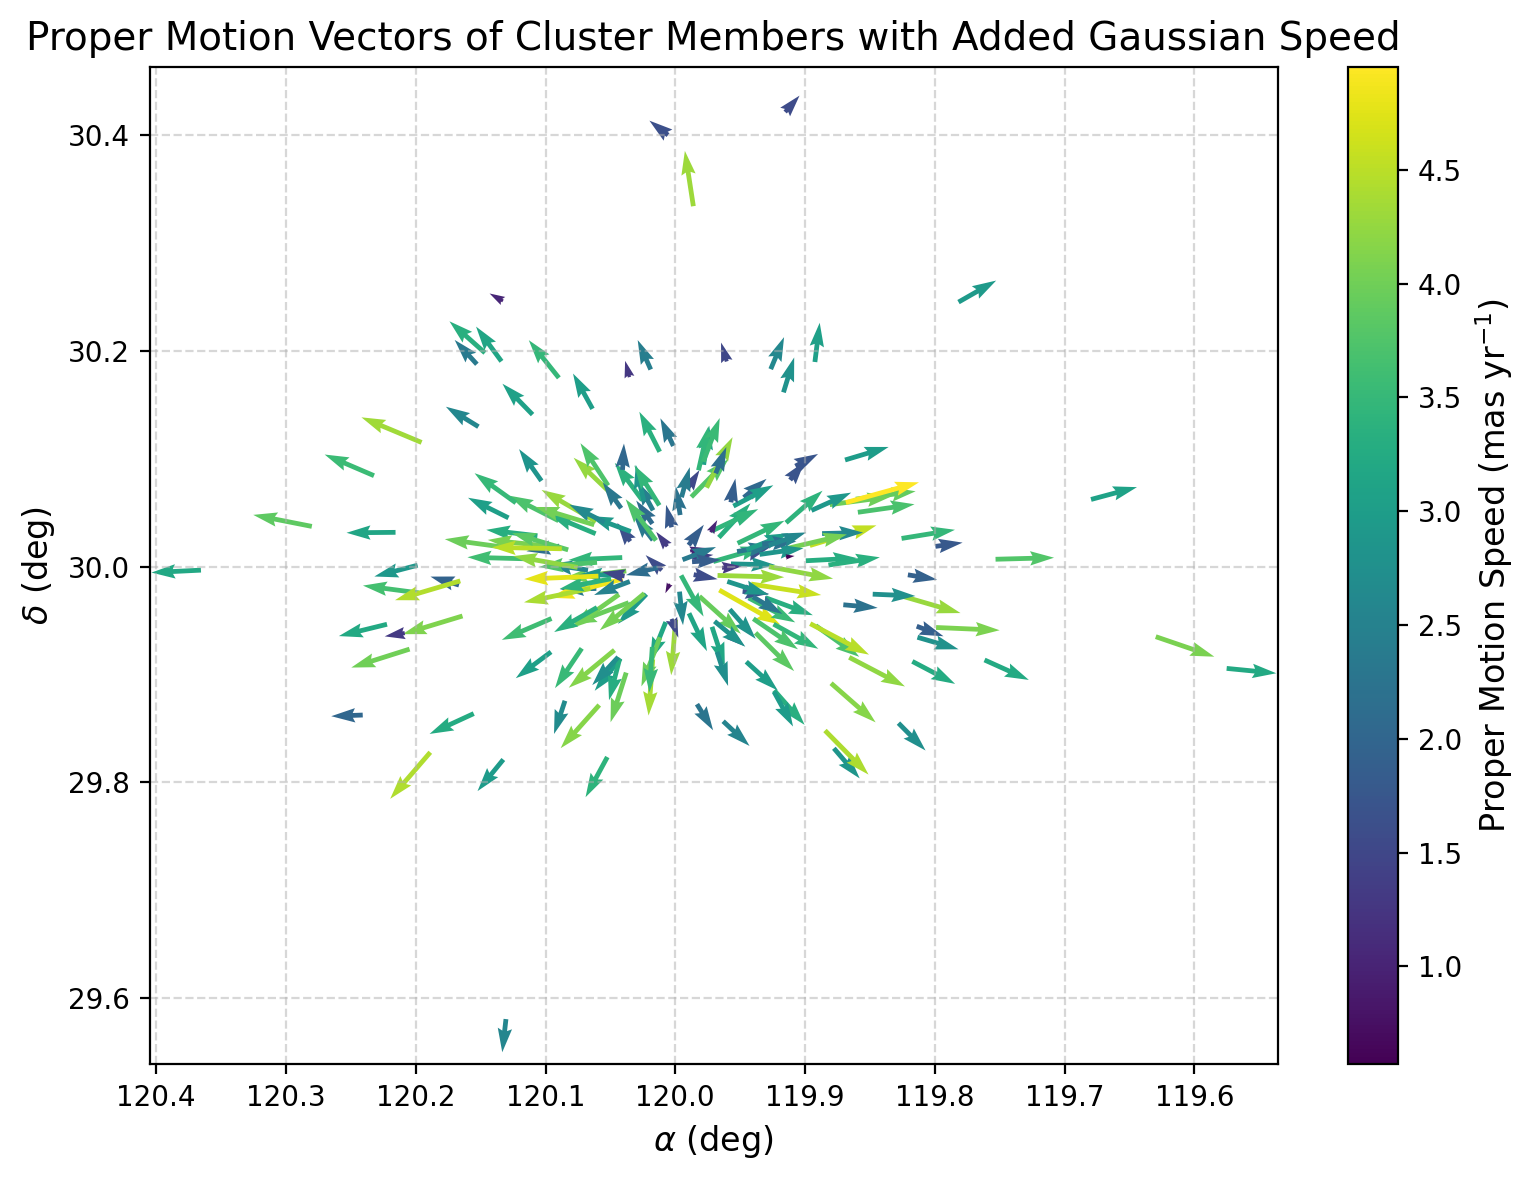
\includegraphics[width=0.5\textwidth]{gaussian-speed.png} % Replace 'example-image' with your image file name
		\caption{} % Add your caption text here
		\label{fig:Gaussian} % Label for referencing the figure
	\end{figure}
	
\end{document}